\documentclass[11pt]{article}

\usepackage[margin=1in]{geometry}
\usepackage[T1]{fontenc}
\usepackage[utf8]{inputenc}
\usepackage{lmodern}
\usepackage{microtype}
\usepackage{amsmath,amssymb,mathtools,bm}
\usepackage{booktabs,array,tabularx}
\usepackage{xcolor}
\usepackage{hyperref}
\usepackage[most]{tcolorbox}
\usepackage{tikz}
\usepackage{pgfplots}
\usepackage{tikz-3dplot}
\usepackage{enumitem}
\usepackage{float}
\usepackage{caption}
\usepackage{fancyhdr}
\usepackage{titlesec}

\pgfplotsset{compat=1.18}
\usetikzlibrary{arrows.meta,calc,positioning,patterns,decorations.pathreplacing,3d,backgrounds,fit}

\definecolor{chapterblue}{HTML}{1F5AA6}
\definecolor{chapterteal}{HTML}{168A8F}
\definecolor{chapterorange}{HTML}{D9822B}
\definecolor{chaptergreen}{HTML}{2D8A4E}
\definecolor{chapterpurple}{HTML}{6B4EAA}
\definecolor{chapterred}{HTML}{B23B3B}
\definecolor{softblue}{HTML}{EAF3FF}
\definecolor{softgreen}{HTML}{EAF8EF}
\definecolor{softorange}{HTML}{FFF4E6}
\definecolor{softpurple}{HTML}{F3EEFF}
\definecolor{softred}{HTML}{FFF0F0}
\definecolor{softgray}{HTML}{F6F7F9}
\definecolor{darkgray}{HTML}{30343B}

\hypersetup{
  colorlinks=true,
  linkcolor=chapterblue,
  urlcolor=chapterblue,
  citecolor=chapterblue,
  pdftitle={Chapter 16. Triple Integrals and Geometry in R3}
}

\setlength{\headheight}{14pt}
\setlength{\parindent}{0pt}
\setlength{\parskip}{0.65em}
\setlist[itemize]{topsep=2pt,itemsep=2pt}
\setlist[enumerate]{topsep=2pt,itemsep=2pt}

\pagestyle{fancy}
\fancyhf{}
\lhead{Chapter 16. Triple Integrals and Geometry in $\mathbb R^3$}
\rhead{\thepage}
\renewcommand{\headrulewidth}{0.4pt}

\titleformat{\section}{\large\bfseries\color{chapterblue}}{\thesection}{0.6em}{}
\titleformat{\subsection}{\normalsize\bfseries\color{darkgray}}{\thesubsection}{0.6em}{}
\renewcommand{\thesection}{16.\arabic{section}}
\renewcommand{\thesubsection}{\thesection.\arabic{subsection}}

\newcommand{\R}{\mathbb R}
\newcommand{\iiintE}{\iiint_E}
\newcommand{\Vol}{\operatorname{Vol}}
\newcommand{\avg}{\operatorname{avg}}
\newcommand{\dd}{\,d}

\newtcolorbox{chapteroverviewbox}{
  enhanced,
  colback=softblue,
  colframe=chapterblue,
  boxrule=0.8pt,
  arc=2mm,
  left=2mm,right=2mm,top=1.5mm,bottom=1.5mm
}

\newtcolorbox{goalbox}{
  enhanced,
  colback=softgreen,
  colframe=chaptergreen,
  title=Learning goals,
  fonttitle=\bfseries,
  boxrule=0.8pt,
  arc=2mm
}

\newtcolorbox{mainideabox}[1][]{
  enhanced,
  colback=softblue,
  colframe=chapterblue,
  title=#1,
  fonttitle=\bfseries,
  boxrule=0.8pt,
  arc=2mm
}

\newtcolorbox{importantbox}[1][]{
  enhanced,
  colback=softred,
  colframe=chapterred,
  title=#1,
  fonttitle=\bfseries,
  boxrule=0.8pt,
  arc=2mm
}

\newtcolorbox{tipbox}[1][]{
  enhanced,
  colback=softgreen,
  colframe=chaptergreen,
  title=#1,
  fonttitle=\bfseries,
  boxrule=0.8pt,
  arc=2mm
}

\newtcolorbox{warningbox}[1][]{
  enhanced,
  colback=softorange,
  colframe=chapterorange,
  title=#1,
  fonttitle=\bfseries,
  boxrule=0.8pt,
  arc=2mm
}

\newcounter{examplecounter}
\newenvironment{workedexample}[1]{%
  \refstepcounter{examplecounter}%
  \begin{tcolorbox}[enhanced,breakable,colback=white,colframe=chapterblue,colbacktitle=chapterblue,
  title={Example 16.\theexamplecounter: #1},fonttitle=\bfseries,boxrule=0.8pt,arc=1.5mm]
}{\end{tcolorbox}}

\tikzset{
  axisline/.style={-Latex,thick,darkgray},
  vector/.style={-Latex,very thick,chapterblue},
  vectorred/.style={-Latex,very thick,chapterred},
  vectorgreen/.style={-Latex,very thick,chaptergreen},
  guide/.style={thin,dashed,gray!65},
  surface/.style={draw=chapterblue!60!black,fill=chapterblue!18,opacity=0.75},
  solidsurface/.style={draw=chapterblue!80!black,fill=chapterblue!20,opacity=0.75},
  topface/.style={draw=chapterorange!80!black,fill=chapterorange!25,opacity=0.85},
  sideface/.style={draw=chapterblue!80!black,fill=chapterblue!18,opacity=0.72},
  baseface/.style={draw=chaptergreen!70!black,fill=chaptergreen!12,opacity=0.55}
}

\begin{document}

\begin{center}
  {\LARGE\bfseries Chapter 16. Triple Integrals and Geometry in $\mathbb R^3$\par}
  \vspace{0.3em}
  {\large Volume, mass, probability, and continuous sums over solid regions\par}
\end{center}

\begin{chapteroverviewbox}
A double integral sums over a two-dimensional region. A triple integral sums over a three-dimensional solid. The change sounds small: replace tiny rectangles by tiny boxes. Conceptually, however, this is a major step. Triple integrals allow us to compute volume, mass, charge, probability, average value, and spatial accumulation over objects in space.

The central geometric skill in this chapter is \textbf{describing a solid region by inequalities}. Once the region is described correctly, the integral is often straightforward. Most errors in triple integrals are not integration errors; they are errors in reading the geometry.

This chapter develops triple integrals in rectangular coordinates. Cylindrical and spherical coordinates are treated in the next chapter. For now, the guiding idea is:
\[
\boxed{\text{A triple integral is a continuous sum over a solid region.}}
\]
\end{chapteroverviewbox}

\begin{goalbox}
After studying this chapter, you should be able to:
\begin{enumerate}
  \item Interpret $\iiint_E f(x,y,z)\,dV$ as a continuous sum over a solid region $E$.
  \item Compute volume as $\iiint_E 1\,dV$.
  \item Set up triple integrals using projections onto coordinate planes.
  \item Describe solids with bounds such as $g_1(x,y)\le z\le g_2(x,y)$.
  \item Change the order of integration in simple three-dimensional regions.
  \item Compute mass, average value, and probability using triple integrals.
  \item Use computation to visualize regions and approximate triple integrals numerically.
\end{enumerate}
\end{goalbox}

\section{From double integrals to triple integrals}

Recall the structure of a double integral over a region $R\subset\R^2$:
\[
\iint_R f(x,y)\,dA.
\]
It is the limit of sums of the form
\[
\sum f(x_{ij}^*,y_{ij}^*)\Delta A.
\]
For a triple integral over a solid region $E\subset\R^3$, we replace area pieces by volume pieces:
\[
\iiint_E f(x,y,z)\,dV=\lim \sum f(x_{ijk}^*,y_{ijk}^*,z_{ijk}^*)\Delta V.
\]
In rectangular coordinates,
\[
\Delta V=\Delta x\,\Delta y\,\Delta z,
\qquad
 dV=dx\,dy\,dz.
\]
For example,
\[
\int_a^b\int_c^d\int_p^q f(x,y,z)\,dz\,dy\,dx
\]
means that we integrate first with respect to $z$, then $y$, then $x$.

\begin{mainideabox}[The guiding picture]
A double integral sums tiny columns above an area region. A triple integral sums tiny boxes inside a solid region.
\end{mainideabox}

\begin{figure}[H]
\centering
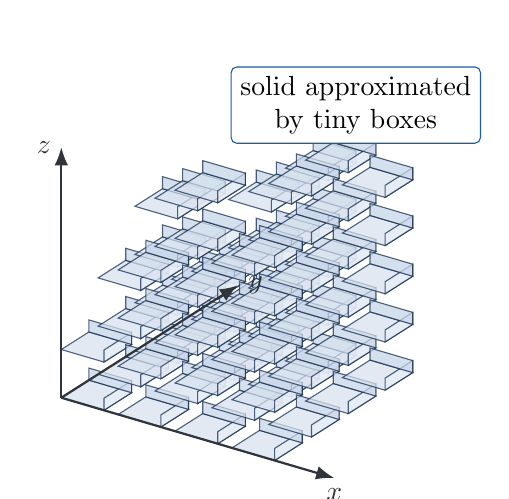
\begin{tikzpicture}[x={(0.85cm,-0.25cm)}, y={(0.55cm,0.35cm)}, z={(0cm,0.72cm)}, scale=0.85]
  \foreach \i in {0,...,3}{
    \foreach \j in {0,...,3}{
      \pgfmathtruncatemacro{\h}{1+mod(\i+\j,3)+\i}
      \foreach \k in {0,...,\h}{
        \draw[draw=chapterblue!45!black,fill=chapterblue!18,opacity=0.72]
          (\i,\j,\k) -- ++(0.75,0,0) -- ++(0,0.75,0) -- ++(-0.75,0,0) -- cycle;
        \draw[draw=chapterblue!45!black,fill=chapterblue!10,opacity=0.72]
          (\i+0.75,\j,\k) -- ++(0,0.75,0) -- ++(0,0,0.25) -- ++(0,-0.75,0) -- cycle;
        \draw[draw=chapterblue!45!black,fill=chapterblue!26,opacity=0.72]
          (\i,\j+0.75,\k) -- ++(0.75,0,0) -- ++(0,0,0.25) -- ++(-0.75,0,0) -- cycle;
      }
    }
  }
  \draw[axisline] (0,0,0) -- (4.8,0,0) node[below] {$x$};
  \draw[axisline] (0,0,0) -- (0,4.8,0) node[right] {$y$};
  \draw[axisline] (0,0,0) -- (0,0,5.2) node[left] {$z$};
  \node[align=center,fill=white,draw=chapterblue,rounded corners=2pt] at (2.2,4.6,4.6)
  {solid approximated\\by tiny boxes};
\end{tikzpicture}
\caption{A solid can be approximated by many small rectangular boxes. A triple integral is the limit of such voxel sums.}
\end{figure}

\section{Volume as a triple integral}

The simplest triple integral occurs when the integrand is $1$.

\begin{importantbox}[Volume of a solid]
If $E\subset\R^3$ is a solid region, then
\[
\Vol(E)=\iiint_E 1\,dV.
\]
\end{importantbox}

This formula says that volume is the sum of all infinitesimal volume elements $dV$ inside the region. It is the three-dimensional analog of
\[
\operatorname{Area}(R)=\iint_R 1\,dA.
\]

\begin{workedexample}{A rectangular box}
Let
\[
E=[0,2]\times[1,4]\times[-1,3].
\]
Then
\[
\Vol(E)=\int_0^2\int_1^4\int_{-1}^3 1\,dz\,dy\,dx.
\]
Evaluate from inside to outside:
\[
\int_{-1}^3 1\,dz=4,
\]
so
\[
\Vol(E)=\int_0^2\int_1^4 4\,dy\,dx=\int_0^2 12\,dx=24.
\]
Of course, the box has side lengths $2$, $3$, and $4$, so the volume is $2\cdot 3\cdot 4=24$.
\end{workedexample}

\begin{figure}[H]
\centering
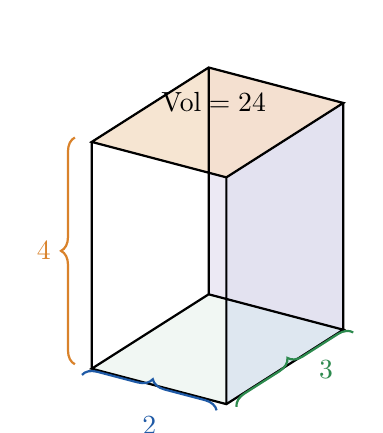
\begin{tikzpicture}[x={(0.95cm,-0.25cm)}, y={(0.55cm,0.35cm)}, z={(0cm,0.8cm)}, scale=0.9]
  \coordinate (O) at (0,0,0);
  \coordinate (A) at (2,0,0);
  \coordinate (B) at (2,3,0);
  \coordinate (C) at (0,3,0);
  \coordinate (D) at (0,0,4);
  \coordinate (E) at (2,0,4);
  \coordinate (F) at (2,3,4);
  \coordinate (G) at (0,3,4);
  \fill[baseface] (O)--(A)--(B)--(C)--cycle;
  \fill[sideface] (A)--(B)--(F)--(E)--cycle;
  \fill[chapterpurple!18,draw=chapterpurple!70!black,opacity=0.7] (C)--(B)--(F)--(G)--cycle;
  \fill[topface] (D)--(E)--(F)--(G)--cycle;
  \draw[thick] (O)--(A)--(B)--(C)--cycle (D)--(E)--(F)--(G)--cycle (O)--(D) (A)--(E) (B)--(F) (C)--(G);
  \draw[decorate,decoration={brace,amplitude=5pt},chapterblue,thick] (0,-0.25,0)--(2,-0.25,0) node[midway,below=5pt] {$2$};
  \draw[decorate,decoration={brace,amplitude=5pt},chaptergreen,thick] (2.15,0,0)--(2.15,3,0) node[midway,right=5pt] {$3$};
  \draw[decorate,decoration={brace,amplitude=5pt},chapterorange,thick] (-0.25,0,0)--(-0.25,0,4) node[midway,left=5pt] {$4$};
  \node at (1,1.4,4.4) {$\Vol=24$};
\end{tikzpicture}
\caption{The triple integral of $1$ over a rectangular box reproduces length times width times height.}
\end{figure}

\section{Solids between two surfaces}

A very common solid has the form
\[
E=\{(x,y,z):(x,y)\in D,\ g_1(x,y)\le z\le g_2(x,y)\}.
\]
Here $D$ is the projection of $E$ onto the $xy$-plane. The solid lies above the lower surface $z=g_1(x,y)$ and below the upper surface $z=g_2(x,y)$. Then
\[
\iiint_E f(x,y,z)\,dV
=\iint_D\left[\int_{g_1(x,y)}^{g_2(x,y)}f(x,y,z)\,dz\right]dA.
\]
If $D$ is a Type I region,
\[
D=\{(x,y):a\le x\le b,\ h_1(x)\le y\le h_2(x)\},
\]
then
\[
\iiint_E f(x,y,z)\,dV
=\int_a^b\int_{h_1(x)}^{h_2(x)}\int_{g_1(x,y)}^{g_2(x,y)}
f(x,y,z)\,dz\,dy\,dx.
\]

\begin{tipbox}[Projection-first method]
To set up a triple integral, first choose a projection plane. Then write the outer two bounds for the projection and the inner bounds for the variable perpendicular to that projection.
\end{tipbox}

\begin{figure}[H]
\centering
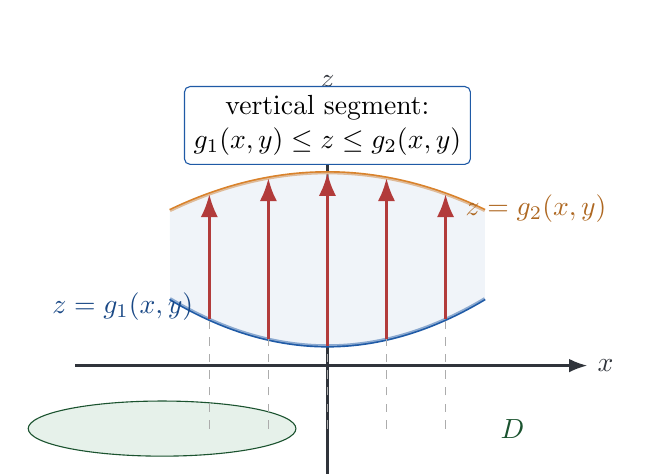
\begin{tikzpicture}[scale=1.0]
  \draw[axisline] (-3.2,0)--(3.3,0) node[right] {$x$};
  \draw[axisline] (0,-1.5)--(0,3.4) node[above] {$z$};
  \fill[chaptergreen!12,draw=chaptergreen!60!black] (-2.1,-0.8) ellipse (1.7 and 0.35);
  \node[chaptergreen!60!black] at (2.35,-0.8) {$D$};
  \draw[very thick,chapterblue,domain=-2:2,samples=120] plot (\x,{0.25+0.15*\x*\x});
  \draw[very thick,chapterorange,domain=-2:2,samples=120] plot (\x,{2.45-0.12*\x*\x});
  \fill[chapterblue!12,opacity=0.55] plot[domain=-2:2,samples=120] (\x,{2.45-0.12*\x*\x}) -- plot[domain=2:-2,samples=120] (\x,{0.25+0.15*\x*\x}) -- cycle;
  \foreach \x in {-1.5,-0.75,0,0.75,1.5}{
    \pgfmathsetmacro{\lo}{0.25+0.15*\x*\x}
    \pgfmathsetmacro{\hi}{2.45-0.12*\x*\x}
    \draw[guide] (\x,-0.8)--(\x,\lo);
    \draw[vectorred] (\x,\lo)--(\x,\hi);
  }
  \node[chapterblue!80!black] at (-2.6,0.75) {$z=g_1(x,y)$};
  \node[chapterorange!80!black] at (2.65,2.0) {$z=g_2(x,y)$};
  \node[align=center,fill=white,draw=chapterblue,rounded corners=2pt] at (0,3.05)
  {vertical segment:\\$g_1(x,y)\le z\le g_2(x,y)$};
\end{tikzpicture}
\caption{A solid between two surfaces is described by a projection region in the $xy$-plane and vertical $z$-bounds.}
\end{figure}

\begin{workedexample}{Volume under a plane over a triangle}
Let $E$ be the tetrahedron in the first octant bounded by the coordinate planes and
\[
x+y+z=1.
\]
The region is
\[
E=\{(x,y,z):x\ge0,\ y\ge0,\ z\ge0,\ x+y+z\le1\}.
\]
Project onto the $xy$-plane. Since $z$ ranges from $0$ to $1-x-y$, the projection is
\[
D=\{(x,y):0\le x\le1,\ 0\le y\le1-x\}.
\]
Thus
\[
\Vol(E)=\int_0^1\int_0^{1-x}\int_0^{1-x-y}1\,dz\,dy\,dx.
\]
Evaluate:
\[
\Vol(E)=\int_0^1\int_0^{1-x}(1-x-y)\,dy\,dx
=\int_0^1\frac{(1-x)^2}{2}\,dx
=\frac16.
\]
\end{workedexample}

\begin{figure}[H]
\centering
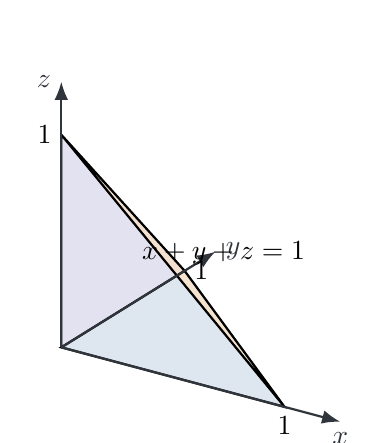
\begin{tikzpicture}[x={(1.05cm,-0.28cm)}, y={(0.58cm,0.36cm)}, z={(0cm,1.0cm)}, scale=2.7]
  \coordinate (O) at (0,0,0);
  \coordinate (X) at (1,0,0);
  \coordinate (Y) at (0,1,0);
  \coordinate (Z) at (0,0,1);
  \fill[baseface] (O)--(X)--(Y)--cycle;
  \fill[sideface] (O)--(X)--(Z)--cycle;
  \fill[chapterpurple!18,draw=chapterpurple!70!black,opacity=0.72] (O)--(Y)--(Z)--cycle;
  \fill[topface] (X)--(Y)--(Z)--cycle;
  \draw[thick] (O)--(X)--(Y)--cycle (O)--(Z) (X)--(Z) (Y)--(Z);
  \draw[axisline] (O)--(1.25,0,0) node[below] {$x$};
  \draw[axisline] (O)--(0,1.25,0) node[right] {$y$};
  \draw[axisline] (O)--(0,0,1.25) node[left] {$z$};
  \node[below] at (X) {$1$};
  \node[right] at (Y) {$1$};
  \node[left] at (Z) {$1$};
  \node at (0.55,0.32,0.48) {$x+y+z=1$};
\end{tikzpicture}
\caption{The tetrahedron $x+y+z\le1$ in the first octant. Its projection onto the $xy$-plane is a triangle.}
\end{figure}

\section{Integrating functions over solids}

Volume is only one example. If $f(x,y,z)$ measures a density, intensity, probability density, energy density, or cost density, then
\[
\iiint_E f(x,y,z)\,dV
\]
sums that quantity over the whole solid.

\begin{workedexample}{A triple integral over the standard tetrahedron}
Evaluate
\[
\iiint_E y\,dV,
\]
where
\[
E=\{(x,y,z):x\ge0,\ y\ge0,\ z\ge0,\ x+y+z\le1\}.
\]
Using the same bounds as before,
\[
\iiint_E y\,dV=\int_0^1\int_0^{1-x}\int_0^{1-x-y} y\,dz\,dy\,dx.
\]
Since $y$ does not depend on $z$,
\[
\int_0^{1-x-y}y\,dz=y(1-x-y).
\]
Thus
\[
\iiint_E y\,dV=\int_0^1\int_0^{1-x}y(1-x-y)\,dy\,dx
=\int_0^1\frac{(1-x)^3}{6}\,dx
=\frac1{24}.
\]
Because of symmetry,
\[
\iiint_E x\,dV=\iiint_E y\,dV=\iiint_E z\,dV=\frac1{24}.
\]
\end{workedexample}

\section{Mass and density in three dimensions}

Suppose an object occupies a solid region $E$ and has density $\rho=\rho(x,y,z)$. The mass of a small box is approximately
\[
\Delta m\approx \rho(x_{ijk}^*,y_{ijk}^*,z_{ijk}^*)\Delta V.
\]
Summing and passing to a limit gives the mass formula.

\begin{importantbox}[Mass from density]
If an object occupies $E\subset\R^3$ and has density $\rho(x,y,z)$, then
\[
M=\iiint_E \rho(x,y,z)\,dV.
\]
\end{importantbox}

\begin{workedexample}{Density increasing with height}
Let $E$ be the box
\[
0\le x\le2,
\qquad
0\le y\le3,
\qquad
0\le z\le1,
\]
and suppose the density is
\[
\rho(x,y,z)=1+z.
\]
Then
\[
M=\int_0^2\int_0^3\int_0^1(1+z)\,dz\,dy\,dx.
\]
First,
\[
\int_0^1(1+z)\,dz=\frac32.
\]
Thus
\[
M=\int_0^2\int_0^3\frac32\,dy\,dx=\int_0^2\frac92\,dx=9.
\]
If the density were constant $1$, the mass would be the volume $6$. Since the density increases with height, the mass is larger.
\end{workedexample}

\begin{figure}[H]
\centering
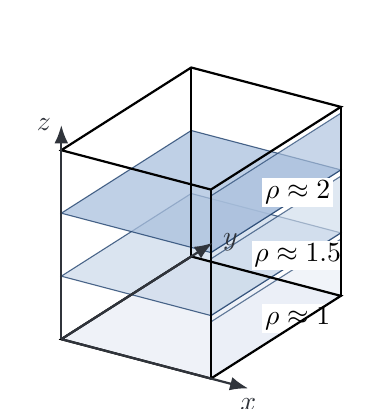
\begin{tikzpicture}[x={(0.95cm,-0.25cm)}, y={(0.55cm,0.35cm)}, z={(0cm,0.8cm)}, scale=1.0]
  \foreach \k/\col/\lab in {0/chapterblue!10/$\rho\approx1$,1/chapterblue!22/$\rho\approx1.5$,2/chapterblue!38/$\rho\approx2$}{
    \fill[draw=chapterblue!60!black,fill=\col,opacity=0.75] (0,0,\k) -- (2,0,\k) -- (2,3,\k) -- (0,3,\k) -- cycle;
    \fill[draw=chapterblue!60!black,fill=\col,opacity=0.65] (2,0,\k) -- (2,3,\k) -- (2,3,{\k+0.9}) -- (2,0,{\k+0.9}) -- cycle;
    \node[fill=white,inner sep=1pt] at (2.35,1.4,{\k+0.45}) {\lab};
  }
  \draw[thick] (0,0,0)--(2,0,0)--(2,3,0)--(0,3,0)--cycle;
  \draw[thick] (0,0,3)--(2,0,3)--(2,3,3)--(0,3,3)--cycle;
  \foreach \p in {(0,0),(2,0),(2,3),(0,3)}{\draw[thick] \p -- ++(0,0,3);}
  \draw[axisline] (0,0,0)--(2.5,0,0) node[below] {$x$};
  \draw[axisline] (0,0,0)--(0,3.5,0) node[right] {$y$};
  \draw[axisline] (0,0,0)--(0,0,3.4) node[left] {$z$};
\end{tikzpicture}
\caption{Density $\rho=1+z$ is larger in higher horizontal layers, so mass exceeds volume.}
\end{figure}

\section{Average value over a solid}

For a function $f(x,y,z)$ on a solid $E$, its average value over $E$ is
\[
f_{\avg}=\frac{1}{\Vol(E)}\iiint_E f(x,y,z)\,dV.
\]
This is the three-dimensional version of the average value of a function over an interval or a plane region.

\begin{workedexample}{Average height in a tetrahedron}
For the standard tetrahedron
\[
E=\{(x,y,z):x,y,z\ge0,\ x+y+z\le1\},
\]
the average value of $z$ is
\[
z_{\avg}=\frac{1}{\Vol(E)}\iiint_E z\,dV.
\]
By symmetry, $\iiint_E z\,dV=1/24$ and $\Vol(E)=1/6$. Therefore
\[
z_{\avg}=\frac{1/24}{1/6}=\frac14.
\]
The centroid of the tetrahedron is
\[
\left(\frac14,\frac14,\frac14\right).
\]
This example previews the role of triple integrals in computing centers of mass.
\end{workedexample}

\section{Other projection directions}

Projection onto the $xy$-plane is common, but not always best. A solid may also be described by projecting onto the $yz$-plane or the $xz$-plane.

\subsection*{Projection onto the $yz$-plane}
If
\[
E=\{(x,y,z):(y,z)\in D,\ g_1(y,z)\le x\le g_2(y,z)\},
\]
then
\[
\iiint_E f(x,y,z)\,dV
=\iint_D\left[\int_{g_1(y,z)}^{g_2(y,z)} f(x,y,z)\,dx\right]dA.
\]

\subsection*{Projection onto the $xz$-plane}
If
\[
E=\{(x,y,z):(x,z)\in D,\ g_1(x,z)\le y\le g_2(x,z)\},
\]
then
\[
\iiint_E f(x,y,z)\,dV
=\iint_D\left[\int_{g_1(x,z)}^{g_2(x,z)} f(x,y,z)\,dy\right]dA.
\]

\begin{warningbox}[Do not choose the projection too early]
A difficult integral often becomes easier if you project in a different direction. Before writing bounds, sketch the solid and ask: which variable naturally runs between two simple surfaces?
\end{warningbox}

\begin{figure}[H]
\centering
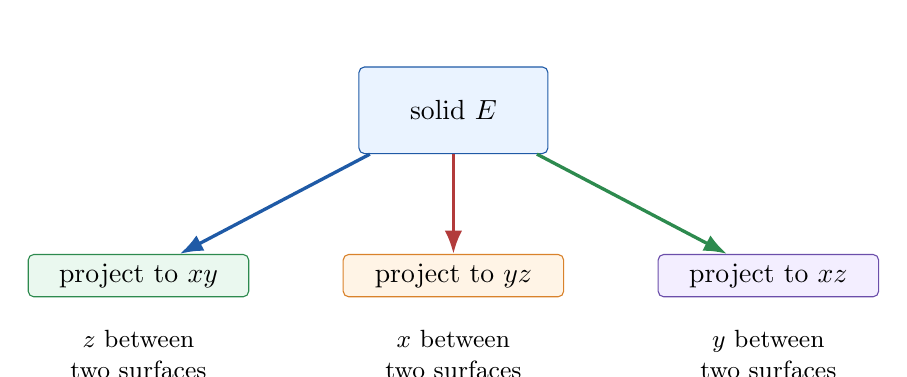
\begin{tikzpicture}[scale=1]
  \node[draw=chapterblue,fill=softblue,rounded corners=2pt,minimum width=2.4cm,minimum height=1.1cm] (solid) at (0,0) {solid $E$};
  \node[draw=chaptergreen,fill=softgreen,rounded corners=2pt,minimum width=2.8cm] (xy) at (-4,-2.1) {project to $xy$};
  \node[draw=chapterorange,fill=softorange,rounded corners=2pt,minimum width=2.8cm] (yz) at (0,-2.1) {project to $yz$};
  \node[draw=chapterpurple,fill=softpurple,rounded corners=2pt,minimum width=2.8cm] (xz) at (4,-2.1) {project to $xz$};
  \draw[vector] (solid) -- (xy);
  \draw[vectorred] (solid) -- (yz);
  \draw[vectorgreen] (solid) -- (xz);
  \node[align=center,font=\small] at (-4,-3.1) {$z$ between\\two surfaces};
  \node[align=center,font=\small] at (0,-3.1) {$x$ between\\two surfaces};
  \node[align=center,font=\small] at (4,-3.1) {$y$ between\\two surfaces};
\end{tikzpicture}
\caption{Projection choice determines which variable becomes the innermost integral.}
\end{figure}

\section{Changing the order of integration}

In double integrals, changing order means rewriting a region in the plane. In triple integrals, changing order means rewriting a solid in space. There are six possible orders:
\[
dz\,dy\,dx,
\qquad dz\,dx\,dy,
\qquad dy\,dz\,dx,
\qquad dy\,dx\,dz,
\qquad dx\,dz\,dy,
\qquad dx\,dy\,dz.
\]
The main principle is simple:
\[
\boxed{\text{The innermost variable describes a line segment through the solid.}}
\]

\begin{workedexample}{The tetrahedron in another order}
For the standard tetrahedron
\[
E=\{(x,y,z):x,y,z\ge0,\ x+y+z\le1\},
\]
we wrote
\[
\iiint_E f(x,y,z)\,dV
=\int_0^1\int_0^{1-x}\int_0^{1-x-y}f(x,y,z)\,dz\,dy\,dx.
\]
Now write the order $dx\,dz\,dy$. For fixed $y$ and $z$,
\[
0\le x\le1-y-z.
\]
The projection onto the $yz$-plane is
\[
0\le y\le1,
\qquad
0\le z\le1-y.
\]
Therefore
\[
\iiint_E f(x,y,z)\,dV
=\int_0^1\int_0^{1-y}\int_0^{1-y-z}f(x,y,z)\,dx\,dz\,dy.
\]
Because the tetrahedron is symmetric, all six orders have similar bounds.
\end{workedexample}

\begin{figure}[H]
\centering
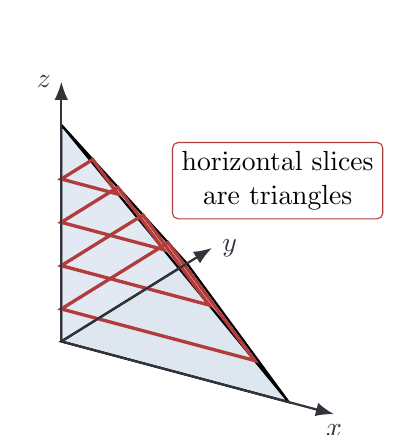
\begin{tikzpicture}[x={(1.05cm,-0.28cm)}, y={(0.58cm,0.36cm)}, z={(0cm,1.0cm)}, scale=2.75]
  \coordinate (O) at (0,0,0);
  \coordinate (X) at (1,0,0);
  \coordinate (Y) at (0,1,0);
  \coordinate (Z) at (0,0,1);
  \fill[baseface] (O)--(X)--(Y)--cycle;
  \fill[sideface] (O)--(X)--(Z)--cycle;
  \fill[topface] (X)--(Y)--(Z)--cycle;
  \draw[thick] (O)--(X)--(Y)--cycle (O)--(Z) (X)--(Z) (Y)--(Z);
  \foreach \zz in {0.15,0.35,0.55,0.75}{
    \pgfmathsetmacro{\a}{1-\zz}
    \draw[very thick,chapterred] (0,0,\zz)--(\a,0,\zz)--(0,\a,\zz)--cycle;
  }
  \draw[axisline] (O)--(1.2,0,0) node[below] {$x$};
  \draw[axisline] (O)--(0,1.2,0) node[right] {$y$};
  \draw[axisline] (O)--(0,0,1.2) node[left] {$z$};
  \node[fill=white,draw=chapterred,rounded corners=2pt,align=center] at (0.62,0.6,0.7)
  {horizontal slices\\are triangles};
\end{tikzpicture}
\caption{Horizontal slices of the first-octant tetrahedron are triangles. Slicing helps rewrite bounds in a new order.}
\end{figure}

\section{Triple integrals and probability}

A joint probability density for three continuous random variables $X,Y,Z$ is a nonnegative function $p(x,y,z)$ such that
\[
\iiint_{\R^3}p(x,y,z)\,dV=1.
\]
For a solid event $E\subset\R^3$,
\[
P((X,Y,Z)\in E)=\iiint_E p(x,y,z)\,dV.
\]
This interpretation is essential in statistics and machine learning. Many models use high-dimensional integrals, but the geometric meaning begins here: probability is accumulated density over a region.

\begin{workedexample}{Uniform distribution in a box}
Suppose $(X,Y,Z)$ is uniformly distributed in the box
\[
0\le x\le2,
\qquad
0\le y\le1,
\qquad
0\le z\le3.
\]
The volume is $6$, so the density is $p(x,y,z)=1/6$ inside the box and $0$ outside. The probability of the sub-box
\[
0\le x\le1,
\qquad
0\le y\le1,
\qquad
1\le z\le3
\]
is
\[
\int_0^1\int_0^1\int_1^3\frac16\,dz\,dy\,dx
=\frac{2}{6}=\frac13.
\]
\end{workedexample}

\section{Numerical triple integration}

In practice, many triple integrals cannot be evaluated exactly. Numerical integration is then necessary. For a rectangular box $[a,b]\times[c,d]\times[p,q]$, a midpoint rule approximation is
\[
\iiint_E f(x,y,z)\,dV
\approx
\sum_{i=1}^m\sum_{j=1}^n\sum_{k=1}^{\ell}
f(\bar x_i,\bar y_j,\bar z_k)\Delta x\Delta y\Delta z.
\]

\begin{figure}[H]
\centering
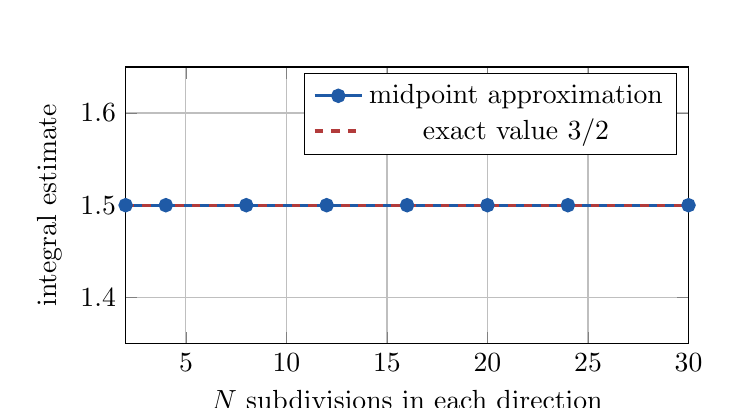
\begin{tikzpicture}
\begin{axis}[
  width=0.72\textwidth,
  height=0.42\textwidth,
  xlabel={$N$ subdivisions in each direction},
  ylabel={integral estimate},
  xmin=2,xmax=30,
  ymin=1.35,ymax=1.65,
  grid=both,
  legend style={at={(0.98,0.98)},anchor=north east,fill=white}
]
\addplot[chapterblue,very thick,mark=*] coordinates {(2,1.50) (4,1.50) (8,1.50) (12,1.50) (16,1.50) (20,1.50) (24,1.50) (30,1.50)};
\addlegendentry{midpoint approximation}
\addplot[chapterred,very thick,dashed] coordinates {(2,1.5) (30,1.5)};
\addlegendentry{exact value $3/2$}
\end{axis}
\end{tikzpicture}
\caption{For $f(x,y,z)=x+y+z$ over the unit cube, the midpoint rule is exact for every grid size because the function is linear.}
\end{figure}

For nonlinear functions, the approximations generally improve as the grid is refined.

\begin{figure}[H]
\centering
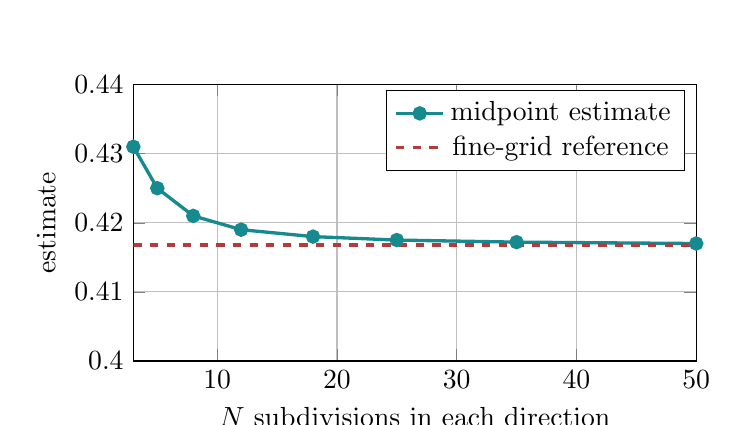
\begin{tikzpicture}
\begin{axis}[
  width=0.72\textwidth,
  height=0.42\textwidth,
  xlabel={$N$ subdivisions in each direction},
  ylabel={estimate},
  xmin=3,xmax=50,
  ymin=0.40,ymax=0.44,
  grid=both,
  legend style={at={(0.98,0.98)},anchor=north east,fill=white}
]
\addplot[chapterteal,very thick,mark=*] coordinates {(3,0.431) (5,0.425) (8,0.421) (12,0.419) (18,0.418) (25,0.4175) (35,0.4172) (50,0.4170)};
\addlegendentry{midpoint estimate}
\addplot[chapterred,very thick,dashed] coordinates {(3,0.4168) (50,0.4168)};
\addlegendentry{fine-grid reference}
\end{axis}
\end{tikzpicture}
\caption{Midpoint approximations for a nonlinear function over the unit cube stabilize as the grid is refined.}
\end{figure}

\section{Monte Carlo integration in three dimensions}

Monte Carlo integration estimates an integral by random sampling. Suppose $E$ is a box of volume $V$ and we want
\[
I=\iiint_E f(x,y,z)\,dV.
\]
If $P_1,\dots,P_N$ are uniformly sampled from $E$, then
\[
I\approx V\cdot \frac1N\sum_{i=1}^N f(P_i).
\]
Monte Carlo methods become especially important in high-dimensional statistics, Bayesian inference, uncertainty quantification, and machine learning.

\begin{figure}[H]
\centering
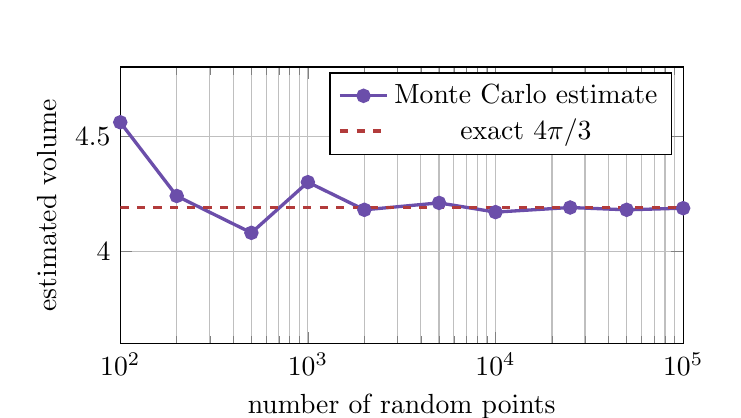
\begin{tikzpicture}
\begin{axis}[
  width=0.72\textwidth,
  height=0.42\textwidth,
  xmode=log,
  xlabel={number of random points},
  ylabel={estimated volume},
  xmin=100,xmax=100000,
  ymin=3.6,ymax=4.8,
  grid=both,
  legend style={at={(0.98,0.98)},anchor=north east,fill=white}
]
\addplot[chapterpurple,very thick,mark=*] coordinates {(100,4.56) (200,4.24) (500,4.08) (1000,4.30) (2000,4.18) (5000,4.21) (10000,4.17) (25000,4.19) (50000,4.18) (100000,4.187)};
\addlegendentry{Monte Carlo estimate}
\addplot[chapterred,very thick,dashed] coordinates {(100,4.18879) (100000,4.18879)};
\addlegendentry{exact $4\pi/3$}
\end{axis}
\end{tikzpicture}
\caption{Monte Carlo estimation of the volume of the unit ball. Random estimates fluctuate but tend to stabilize with many samples.}
\end{figure}

\section{Moments and centers of mass}

Triple integrals also compute balance points. Suppose an object occupies $E$ with density $\rho(x,y,z)$ and mass
\[
M=\iiint_E \rho(x,y,z)\,dV.
\]
The moments about the coordinate planes are
\[
M_{yz}=\iiint_E x\rho(x,y,z)\,dV,
\qquad
M_{xz}=\iiint_E y\rho(x,y,z)\,dV,
\qquad
M_{xy}=\iiint_E z\rho(x,y,z)\,dV.
\]
The center of mass is
\[
(\bar x,\bar y,\bar z)=\left(\frac{M_{yz}}{M},\frac{M_{xz}}{M},\frac{M_{xy}}{M}\right).
\]
If $\rho$ is constant, the center of mass is the centroid of the region.

\begin{workedexample}{Centroid of the standard tetrahedron}
For the standard tetrahedron, by symmetry and the computation above,
\[
\bar x=\bar y=\bar z=\frac14.
\]
Thus the centroid is
\[
\left(\frac14,\frac14,\frac14\right).
\]
This point is closer to the origin than to the opposite face because the tetrahedron is widest near the coordinate planes.
\end{workedexample}

\begin{figure}[H]
\centering
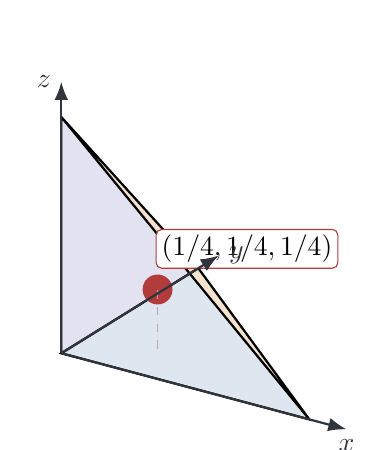
\begin{tikzpicture}[x={(1.05cm,-0.28cm)}, y={(0.58cm,0.36cm)}, z={(0cm,1.0cm)}, scale=3]
  \coordinate (O) at (0,0,0);
  \coordinate (X) at (1,0,0);
  \coordinate (Y) at (0,1,0);
  \coordinate (Z) at (0,0,1);
  \fill[baseface] (O)--(X)--(Y)--cycle;
  \fill[sideface] (O)--(X)--(Z)--cycle;
  \fill[chapterpurple!18,draw=chapterpurple!70!black,opacity=0.72] (O)--(Y)--(Z)--cycle;
  \fill[topface] (X)--(Y)--(Z)--cycle;
  \draw[thick] (O)--(X)--(Y)--cycle (O)--(Z) (X)--(Z) (Y)--(Z);
  \fill[chapterred] (0.25,0.25,0.25) circle (1.8pt);
  \node[fill=white,draw=chapterred,rounded corners=2pt,inner sep=2pt] at (0.5,0.45,0.42) {$(1/4,1/4,1/4)$};
  \draw[guide] (0.25,0.25,0)--(0.25,0.25,0.25);
  \draw[axisline] (O)--(1.15,0,0) node[below] {$x$};
  \draw[axisline] (O)--(0,1.15,0) node[right] {$y$};
  \draw[axisline] (O)--(0,0,1.15) node[left] {$z$};
\end{tikzpicture}
\caption{The centroid of the first-octant tetrahedron is $(1/4,1/4,1/4)$.}
\end{figure}

\section{Triple integrals in the age of data and AI}

Triple integrals appear naturally in modern applied mathematics, statistics, and machine learning.

\subsection*{Spatial data and voxel models}
Medical imaging, climate models, fluid simulations, and three-dimensional computer vision often represent space using voxels. A voxel is a small three-dimensional box. A triple integral is the mathematical limit of summing quantities over voxels.

Examples include total mass in a scanned object, total heat in a region, average intensity in a three-dimensional image, and probability that a random spatial point lies in a target region.

\subsection*{Probability and Bayesian inference}
For three parameters $\theta_1,\theta_2,\theta_3$, a posterior density $p(\theta_1,\theta_2,\theta_3\mid \text{data})$ satisfies
\[
\iiint p(\theta_1,\theta_2,\theta_3\mid \text{data})\,d\theta_1\,d\theta_2\,d\theta_3=1.
\]
A probability statement about the parameters is a triple integral over a region in parameter space.

\subsection*{Continuous loss and risk}
In statistical learning, expected loss may be written as an integral over feature space. In three variables, a risk functional may look like
\[
R(w)=\iiint L(w;x,y,z)p(x,y,z)\,dV.
\]
This is a triple integral of loss weighted by a probability density.

\section{Common mistakes}

\begin{warningbox}[Mistake 1: Forgetting the projection]
Bounds such as $0\le z\le g(x,y)$ are incomplete unless the allowed $(x,y)$ values are described.
\end{warningbox}

\begin{warningbox}[Mistake 2: Using the wrong upper surface]
Always check which surface is above on the projection region.
\end{warningbox}

\begin{warningbox}[Mistake 3: Mixing the order of bounds and differentials]
In $dz\,dy\,dx$, the $z$-bounds come first, then $y$-bounds, then $x$-bounds.
\end{warningbox}

\begin{warningbox}[Mistake 4: Treating dependent variables as constants incorrectly]
When integrating with respect to $z$, expressions involving $x$ and $y$ are constant, but the $z$-bounds may depend on $x$ and $y$.
\end{warningbox}

\begin{warningbox}[Mistake 5: Assuming every solid is a box]
Most real regions require variable bounds.
\end{warningbox}

\begin{warningbox}[Mistake 6: Not checking units]
If $f$ has units of density, then $f\,dV$ has units of mass.
\end{warningbox}

\section{Summary}

A triple integral is a continuous sum over a solid region:
\[
\iiint_E f(x,y,z)\,dV.
\]
The most important special cases are:
\[
\Vol(E)=\iiint_E1\,dV,
\qquad
M=\iiint_E\rho(x,y,z)\,dV,
\qquad
f_{\avg}=\frac{1}{\Vol(E)}\iiint_E f(x,y,z)\,dV.
\]
The most common rectangular-coordinate setup is
\[
E=\{(x,y,z):(x,y)\in D,\ g_1(x,y)\le z\le g_2(x,y)\},
\]
which gives
\[
\iiint_E f(x,y,z)\,dV
=\iint_D\left[\int_{g_1(x,y)}^{g_2(x,y)} f(x,y,z)\,dz\right]dA.
\]
The key skill is not merely integration. The key skill is \textbf{turning geometry into correct bounds}.

\section*{Exercises}
\addcontentsline{toc}{section}{Exercises}

\subsection*{Conceptual exercises}
\begin{enumerate}
  \item Explain why $\iiint_E1\,dV$ gives the volume of $E$.
  \item What is the projection of a solid onto the $xy$-plane?
  \item In the integral
  \[
  \int_0^2\int_0^{4-x}\int_{x+y}^{5}f(x,y,z)\,dz\,dy\,dx,
  \]
  describe the solid region in words.
  \item Why might it be easier to project a region onto the $yz$-plane instead of the $xy$-plane?
  \item Explain the difference between mass and volume in terms of triple integrals.
  \item What does it mean for $p(x,y,z)$ to be a joint probability density?
\end{enumerate}

\subsection*{Computational exercises}
\begin{enumerate}[start=7]
  \item Evaluate $\int_0^1\int_0^2\int_0^3(x+y+z)\,dz\,dy\,dx$.
  \item Find the volume of the box $-1\le x\le2$, $0\le y\le4$, $1\le z\le5$.
  \item Evaluate $\int_0^1\int_0^{1-x}\int_0^{1-x-y}1\,dz\,dy\,dx$.
  \item Evaluate $\int_0^1\int_0^{1-x}\int_0^{1-x-y}x\,dz\,dy\,dx$.
  \item Let $E$ be the solid under $z=4-x^2-y^2$ and above the rectangle $0\le x\le1$, $0\le y\le1$. Set up a triple integral for the volume of $E$.
  \item Let $E$ be the solid between $z=x^2+y^2$ and $z=4$. Set up the volume integral in rectangular coordinates using projection onto the $xy$-plane. Do not evaluate.
  \item Let $E$ be the tetrahedron $x,y,z\ge0$, $x+y+z\le2$. Find its volume.
  \item Let $E=[0,1]^3$ and $\rho(x,y,z)=1+x+y+z$. Find the mass of $E$.
  \item Find the average value of $f(x,y,z)=z$ over the unit cube $[0,1]^3$.
\end{enumerate}

\subsection*{Geometry and setup exercises}
\begin{enumerate}[start=16]
  \item Describe the solid represented by
  \[
  0\le x\le1,
  \qquad
  0\le y\le1-x,
  \qquad
  0\le z\le2-x-y.
  \]
  \item Rewrite the tetrahedron integral
  \[
  \int_0^1\int_0^{1-x}\int_0^{1-x-y} f(x,y,z)\,dz\,dy\,dx
  \]
  in the order $dy\,dz\,dx$.
  \item Set up, but do not evaluate, an integral for the volume of the solid above $z=0$, below $z=9-x^2-y^2$, and above the first quadrant of the $xy$-plane.
  \item Set up a triple integral for the mass of the solid in Exercise 18 if $\rho(x,y,z)=z+1$.
  \item Let $E$ be the region bounded by $z=0$, $z=1-y$, $x=0$, $x=2$, and $y=0$. Write $\iiint_E f(x,y,z)\,dV$ as an iterated integral.
\end{enumerate}

\subsection*{Computational lab exercises}
\begin{enumerate}[start=21]
  \item Use a midpoint rule on a grid to approximate
  \[
  \int_0^1\int_0^1\int_0^1 e^{-(x^2+y^2+z^2)}\,dV.
  \]
  \item Use random sampling to estimate the volume of the region $x^2+y^2+z^2\le1$.
  \item Use random sampling to estimate the volume of the tetrahedron $x,y,z\ge0$, $x+y+z\le1$.
  \item Plot horizontal slices of the solid under $z=4-x^2-y^2$ and above the $xy$-plane.
  \item Write a function that estimates $\iiint_E f\,dV$ over a box using the midpoint rule.
\end{enumerate}

\section*{Python lab}
\addcontentsline{toc}{section}{Python lab}

A companion Python lab for this chapter should include:
\begin{itemize}
  \item plotting basic solid regions,
  \item voxel approximations of volume,
  \item midpoint approximation for triple integrals,
  \item Monte Carlo estimation of volumes,
  \item probability integrals over 3D regions,
  \item center-of-mass computations for simple solids.
\end{itemize}

\end{document}
